\documentclass[10pt,draftclsnofoot,onecolumn]{IEEEtran}
\usepackage[margin=0.75in]{geometry}
\usepackage{listings}
\usepackage{underscore}
\usepackage[breaklinks]{hyperref}
\usepackage{url}
\usepackage{breakurl}
\usepackage{graphicx}
\usepackage{atbegshi}% http://ctan.org/pkg/atbegshi
\usepackage{color}
\usepackage{rotating}

\renewcommand{\refname}{References}
\definecolor{lightgray}{rgb}{.9,.9,.9}
\definecolor{darkgray}{rgb}{.4,.4,.4}
\definecolor{purple}{rgb}{0.65, 0.12, 0.82}

\lstdefinelanguage{JavaScript}{
  keywords={typeof, new, true, false, catch, function, return, null, catch, switch, var, if, in, while, do, else, case, break},
  keywordstyle=\color{blue}\bfseries,
  ndkeywords={class, export, boolean, throw, implements, import, this},
  ndkeywordstyle=\color{darkgray}\bfseries,
  identifierstyle=\color{black},
  sensitive=false,
  comment=[l]{//},
  morecomment=[s]{/*}{*/},
  commentstyle=\color{purple}\ttfamily,
  stringstyle=\color{red}\ttfamily,
  morestring=[b]',
  morestring=[b]"
}

\lstset{
   language=Python,
   backgroundcolor=\color{lightgray},
   extendedchars=true,
   basicstyle=\footnotesize\ttfamily,
   showstringspaces=false,
   showspaces=false,
   numbers=left,
   numberstyle=\footnotesize,
   numbersep=9pt,
   tabsize=2,
   breaklines=true,
   showtabs=false,
   captionpos=b
}

\hypersetup{
    bookmarks=false, % show bookmarks bar?
    pdftitle={Final Report }, % title
    pdfauthor={Malcom Diller, Evan Steele, Sean Rettig}, % author
    pdfsubject={Raspberry Pi Outdoor Lighting}, % subject of the document
    pdfkeywords={TeX, LaTeX, graphics, images}, % list of keywords
    colorlinks=true, % false: boxed links; true: colored links
    linkcolor=blue, % color of internal links
    citecolor=black, % color of links to bibliography
    filecolor=black, % color of file links
    urlcolor=blue, % color of external links
  %linktoc=page % only page is linked
}
\title{Not Exactly the Internet of Things for Outdoor Lighting\\ Spring Term 2016 Report\\ Final Stage}
\author{Oregon State University CS Senior Capstone Group 22\\Malcolm Diller (dillerm@oregonstate.edu), Sean Rettig (rettigs@oregonstate.edu), Evan Steele (steelee@oregonstate.edu)\\Client: Victor Hsu (hsuv@onid.orst.edu)}

\begin{document}
\maketitle
\begin{abstract}

``Not Exactly the Internet of Things for Outdoor Lighting'' (or simply
``PiLight'') is a self-contained home lighting automation system designed to be
powerful and highly customizable, yet inexpensive.  Standard wallwart plug
timers are cheap, but their usefulness is limited.  High-tech
Internet-connected automation systems are feature-rich, but are often very
expensive, are not easily customizable, and can be rendered useless if the
external service is ever shut down.  PiLight solves this issue by not requiring
any external dependencies to function normally.  Furthermore, PiLight is built
from commodity hardware and open source software, so the system is not only
inexpensive, but also easy to extend and personalize, for the technically
inclined.  PiLight includes a sophisticated rule and scheduling system and has
the potential to integrate with devices other than lights, such as sprinkler
systems, garage door openers, and more.

\end{abstract}
\newpage
\tableofcontents
\newpage
\section{Introduction}
``Not Exactly the Internet of Things for Outdoor Lighting'' (or simply
``PiLight'') is a self-contained home lighting automation system designed to be
powerful and highly customizable, yet inexpensive.  Originally commissioned by
Victor Hsu at Oregon State University for simple outdoor lighting automation,
the project has expanded to include a sophisticated rule and scheduling system
and has the potential to integrate with devices other than lights, such as
sprinkler systems, garage door openers, and more.

While similar products do exist, PiLight attempts to fill a niche between
``overly simplistic'' and ``walled garden''.  Standard wallwart plug timers are
cheap, but their usefulness is limited; if you want your lights to turn on at
sunset, for example, you must manually adjust the timer throughout the year.
If you only want your lights on for the weekends, you're out of luck.
High-tech Internet-connected automation systems are feature-rich, but are often
very expensive and not easily customizable.  Even worse, should the external
Internet services running the show break or shut down, the entire system can be
rendered useless.  PiLight solves these issues by being self-contained; no
external dependencies are required for the system to function normally.
Furthermore, PiLight is built from commodity hardware and open source software,
so the system is not only inexpensive, but also easy to extend and personalize,
for the technically inclined.

PiLight consists of a wireless network of tiny ``client'' computers that each
control up to 4 sets of lights and are controlled by a central ``server''
computer, which automatically sends out commands to the clients when it's time
to turn on or off.  The central node runs a control program that can be easily
accessed via a touch screen, a web browser, or a mobile device, where the user
can locally or remotely control each light individually. The control interface
allows users to easily set ``rules'' for what their lights do and when,
depending on the time of day, day of the week, sun position, and potentially
even triggers such as weather conditions or calendar dates.

A Raspberry Pi with a small touchscreen and Wi-Fi card comprises the central
control unit; it runs its own web server to allow control of lights, as well as
a wireless network that allows both users and client nodes to connect.  The
client nodes are each composed of an ESP8266 Wi-Fi module and a relay, which
automatically connect to the Pi's wireless network when the ``Add Devices''
button is pressed on the web UI.  In a commercial implementation of PiLight,
the client nodes could be integrated into a standard power strip/surge
protector, so users can simply plug their devices in and start using the system
immediately without having to order and wire up the components individually.

The PiLight team is composed of Malcolm Diller, Sean Rettig, and Evan Steele,
who are computer science students at Oregon State University.  Evan Steele's
primary role was creating the Yocto Linux builds for the Raspberry Pi and
writing the ESP8266 firmware, while Malcolm and Sean focused primarily on the
web application, a Flask app with a Bootstrap frontend.  In particular, Sean
developed most of the rule system and advanced settings for lights, while
Malcolm and Evan developed the front page UI, using Javascript to dynamically
update the statuses and names of lights.  Throughout development, we have met
with our client, Victor, to help clarify project requirements, drive
hardware/software design decisions, and provide general guidance to ensure the
project's success.

\section{Original Requirements Document}
\subsection{Team}

\subsubsection{Team Name}

Cupcake Warriors

\subsubsection{Team Members} \hfill

\begin{tabular}{ l l }
    Malcolm Diller & dillerm@oregonstate.edu\\
    Sean Rettig & rettigs@oregonstate.edu\\
    Evan Steele & steelee@oregonstate.edu\\
\end{tabular}
\hfill\break

\subsubsection{Client} \hfill

\begin{tabular}{ l }
    Victor Hsu\\
    Oregon State University\\
    Phone: 541-737-4398\\
    Email: hsuv@onid.orst.edu
\end{tabular}
\hfill\break

\subsection{Introduction}

\subsubsection{Problem Statement}

Outdoor lighting seems like a simple problem to solve, but the solutions on the
market today are less than ideal.  The standard transformer/timer combos
available in the big box stores are rudimentary and clunky at best (constantly
needing to be adjusted for the changing sunset and sunrise times), but are
reasonably priced. The new-generation smart apps for home automation are
flexible and fancier, but are quite spendy and lock you into a specific
protocol.  So why not use an open platform running on commodity hardware?  Easy
to use, reasonably priced, and highly customizable--that is our goal.

\subsubsection{Project Description}

Our system will consist of a wireless network of tiny ``client'' computers that
each control up to 4 sets of lights and are controlled by a central ``server''
computer, which will automatically send out commands to the clients when it's
time to turn on or off.  The central node will run a control program that can
be easily accessed via a touch screen, a web browser, or a mobile device, where
the user can locally or remotely control each light individually.  Want your
lights to turn on at sunset and then dim gradually as the sun rises?  Simple.
Want your lights to flash when you're throwing a party?  Just press a button.
The control interface will allow users to easily set ``rules'' for what their
lights do and when, depending on the time of day, the sun/moon position, and
potentially even triggers such as weather conditions or calendar dates.  This
system will be easily extensible to potentially control other devices as well,
such as garage doors, sound systems, and more.

\subsubsection{Design}

Specifically, we plan to use a Raspberry Pi running Linux as the central server
computer.  The Raspberry Pi will run a web server program that will allow
nearby devices (such as laptops, phones, or tablets) to control it over a
wireless network, or if connected to the home's internet connection, from
practically anywhere in the world.  The Pi will also have a small touchscreen
connected to it with the website open in a browser, so the user has a dedicated
interface for the device.  The Pi will connect wirelessly to small wifi-enabled
microcontrollers placed throughout the home, each of which are connected to up
to 4 relays to control 4 sets of lights.

\subsection{Requirements}

\subsubsection{Critical Requirements}

The following requirements are critical to the basic functionality of the
system and must be functional prior to the expo in spring term.

\begin{enumerate}
    \item Device control
        \begin{enumerate}
            \item Server is loaded with Linux and is able to boot up to a
                graphical interface that can be viewed and controlled by the
                device's touchscreen.
            \item Server is able to start the server control program
                automatically when powered on.
            \item Clients are loaded with the client control program, which
                runs automatically when the device is powered on.
            \item Client control program is able to automatically discover
                relays/lights that are connected to it.
            \item Client control program can control the relays to power the
                lights on/off individually.
            \item Lights can be toggled over a user-specified period of time,
                e.g. a light can gradually turn on and grow brighter over the
                course of 30 seconds.
            \item Server is able to act as a wireless access point that each
                client can connect to.
            \item Clients can be paired with a server by putting the server
                into ``pairing mode'' (by pressing a button either on the user
                interface or on the Pi itself) that will last for a short time
                (just a few seconds). The server will then wirelessly broadcast
                UDP packets that nearby unpaired clients will see and use to
                connect to the server. This system will allow multiple servers
                to be used in close proximity with separate sets of clients.
            \item Clients are able to communicate to the server which lights
                are available for control.
            \item Server is able to send light toggle instructions wirelessly
                to clients.
            \item Clients are able to read light toggle instructions wirelessly
                from the server.
            \item Clients are able to perform light toggle instructions
                received from the server.
        \end{enumerate}

    \item User interface
        \begin{enumerate}
            \item Main control program on server serves a web site with a
                control interface for the user.
            \item The web interface is accessible via the system's built-in
                touchscreen.
            \item The web interface is accessible to other devices like laptops
                and phones via a local wireless network.
            \item The web interface displays a list of connected clients.
            \item The web interface allows users to give each client a
                ``nickname'' for easy identification.
            \item The web interface displays a list of connected lights.
            \item The web interface allows users to give each light a
                ``nickname'' for easy identification.
            \item The web interface contains buttons for each light that can be
                used to toggle lights individually.
            \item The web interface contains sliders for each light that can be
                used to change the intensity of lights individually.
            \item The web interface contains the ability to put lights into
                ``groups'' that can be controlled together all at once.
            \item The web interface displays a list of light groups.
            \item The web interface allows users to give each light group a
                ``nickname'' for easy identification.
            \item Groups can also be nested into other groups to create
                hierarchies of lights.  For example, there can be two groups
                called ``Front Porch'' and ``Back Porch'' that control the
                front and back porch lights, respectively.  Both groups can
                then be inside another group called ``House''.  If the
                ``House'' group is toggled on, then both the front and back
                porch lights will be toggled on.  If just the front porch
                lights are then toggled off, the back lights will stay on.
            \item The web interface provides the user with options to toggle
                lights/groups based on rules, as described in the below
                ``Rules'' section.
        \end{enumerate}

    \item Rules
        \begin{enumerate}
            \item Lights can be toggled manually, overriding any rules (as
                described in the previous section). The manual setting will
                stay in effect until another rule is triggered. For example, if
                your lights are set to turn off every morning at 6am, but you
                manually turn them on at 7am, they will stay on all day until
                the next morning at 6am.
            \item Rules can be toggled manually to temporarily disable them.
                For example, if you have your lights set to turn on every night
                at 8pm, but are going on vacation for a week and don't need
                them, you can turn that rule off and it will stop triggering
                until you turn it on again, keeping the lights off until after
                you get back. This way, the rule doesn't need to be deleted and
                completely recreated from scratch.
            \item Lights can be toggled based on time of day (e.g. ``turn on at
                8pm and turn off at 6am'').
            \item Lights can be toggled based on day of week (e.g. ``turn on
                during Wednesdays'').
            \item Lights can be toggled based on day of month (e.g. ``turn on
                every 1st of the month'').
            \item Lights can be toggled based on day of year (e.g. ``turn on
                every January 1st'').
            \item Lights can be toggled based on specific dates (e.g. ``turn on
                from Dec. 24th at 2am to Dec 27th at 8pm'').
            \item Lights can be toggled based on sunrise/sunset times (using
                sunset/sunrise times either preloaded onto the Pi or retrieved
                from an Internet service, and using a geograpic location either
                entered by the user or determined through an Internet service)
            \item Multiple rules can be applied to a single light/group using
                an AND/OR system to combine the rules (e.g. ``turn on between
                8pm and 6am AND turn on on Wednesday'' will turn the lights on
                between 8pm and 6am on Wednesdays, and will be off the rest of
                the time, whereas using an OR instead of an AND would cause the
                lights to be on every day from 8pm to 6am and also on all day
                during Wednesday).
            \item Lights can be toggled based on the toggle state of its parent
                group (e.g. by default, a light will turn on if its parent
                group turns on, but it can also be set to turn off if the
                parent group turns on).
            \item Rules can be set to toggle early/late by a constant or random
                period of time.  For example, lights can be configured to turn
                on exactly 30 minutes after sunset, or perhaps randomly between
                6pm and 6:30pm.
            \item Lights within a group can be set to individually toggle
                early/late by a random period of time so that they toggle in a
                staggered fashion.  For example, if there are 5 lights in a
                group and are set to toggle off at 8pm, you can have the first
                light randomly toggle a few seconds before 8pm, then the next a
                few seconds later, etc. in a random order and with randomized
                times.
            \item Lights/groups can be set to gradually dim/brighten over a set
                period of time.  For example, lights can turn on and gradually
                brighten from sunset to 30 minutes after sunset, after which
                they are at full brightness.
        \end{enumerate}
\end{enumerate}

\subsubsection{Stretch Goals}

The following requirements are optional; they are not critical to the basic
functionality of the system and may be implemented only if time permits.

\begin{enumerate}[resume]
    \item Device control
        \begin{enumerate}
            \item System also controls devices other than lights
                \begin{enumerate}
                    \item Garage door openers (e.g. users can program their
                        garage door to automatically close at night).
                    \item Music players (e.g. users can set music to
                        automatically play in the evenings from an attached
                        music player or from the Internet).
                    \item Holiday decorations (e.g. users can set snowglobes or
                        animatronic deer to automatically turn on at night)
                    \item Sprinkler systems (e.g. users can set their
                        sprinklers to turn on from 4am to 5am).
                \end{enumerate}
        \end{enumerate}
    \item User interface
        \begin{enumerate}
            \item The web interface is accessible over the Internet (i.e. the
                user can control the system from anywhere in the world with an
                Internet connection, not just at their home)
                \begin{enumerate}
                    \item The web interface is accessible only to the homeowner
                        or other authorized individuals (to prevent the general
                        public from being able to view/control the user's
                        lights).  This could be implemented by asking the user
                        to provide a password when logging into the system for
                        the first time from a particular device.  The device
                        could then stay logged in via a cookie until the user
                        logs out.
                    \item The web interface is hosted on a remote server for
                        high availablity and the lack of need for the user to
                        perform port forwarding on their router.  If the web
                        server is running on the user's existing home network,
                        the site won't be available unless the user manually
                        opens their router's interface and creates a port
                        forwarding rule, and also won't be available in the
                        case that the user's router/modem loses power or
                        connection to the Internet.  If the site was hosted
                        externally, the user would still be able to view how
                        the system is currently set up and make changes that
                        will apply once the user's power and/or Internet
                        connection are restored.
                \end{enumerate}
        \end{enumerate}
    \item Rules
        \begin{enumerate}
            \item Lights can be toggled based on weather conditions (e.g.
                lights can turn on automatically if it starts raining).  This
                would require an Internet connection or light/moisture sensors.
            \item Lights can be toggled based on a schedule in the user's
                calendar (e.g. a user could create a lighting schedule on their
                Google calendar and it would ``sync'' with the lighting
                system).  This would require Internet connection.
            \item Lights can be toggled based on moon position or other
                celestial data (e.g. lights could turn off during a full moon
                or solar eclipse for better viewing).  This would likely
                require either an Internet connection or a cache of preloaded
                data and the user's location.
            \item Lights can be toggled based on input from attached sensors
                \begin{enumerate}
                    \item Motion sensors (e.g. lights turn on when someone
                        walks up to the front door)
                    \item Light sensors (e.g. lights turn off at a certain
                        brightness level, regardless of time of day, weather,
                        moon phase, etc.  This would also account for an area's
                        brightness changing with the seasons and tree cover).
                    \item Moisture sensors (e.g. lights turn on when it's wet
                        outside, negating the need for an Internet connection
                        to determine if it's raining andpossibly providing more
                        accurate results.  Could also potentially be used in
                        combination with sprinkler integration to stop watering
                        once a certain moisture level has been reached).
                    \item Sound sensors (e.g. lights turn on after a loud
                        noise, or can strobe according to the beat of music
                        that is playing).
                \end{enumerate}
        \end{enumerate}
\end{enumerate}

\subsection{Preliminary Timetable}

By the end of fall term, we plan to have a working proof-of-concept, using the
Raspberry Pi and a basic control program to toggle lights on and off.  By the
end of winter term, we plan to have all required features at least partially
implemented, at which our project enters the beta phase.  As we finish up by
ironing out bugs and perhaps completing stretch goals, we will release version
1.0 prior to the expo.

\subsubsection{Gantt Chart}
Gantt chart available at our project SharePoint website:
\url{https://oregonstateuniversity-my.sharepoint.com/personal/rettigs_oregonstate_edu/capstone22_project/_layouts/15/start.aspx#/Lists/Tasks/gantt.aspx}
\begin{sidewaysfigure}
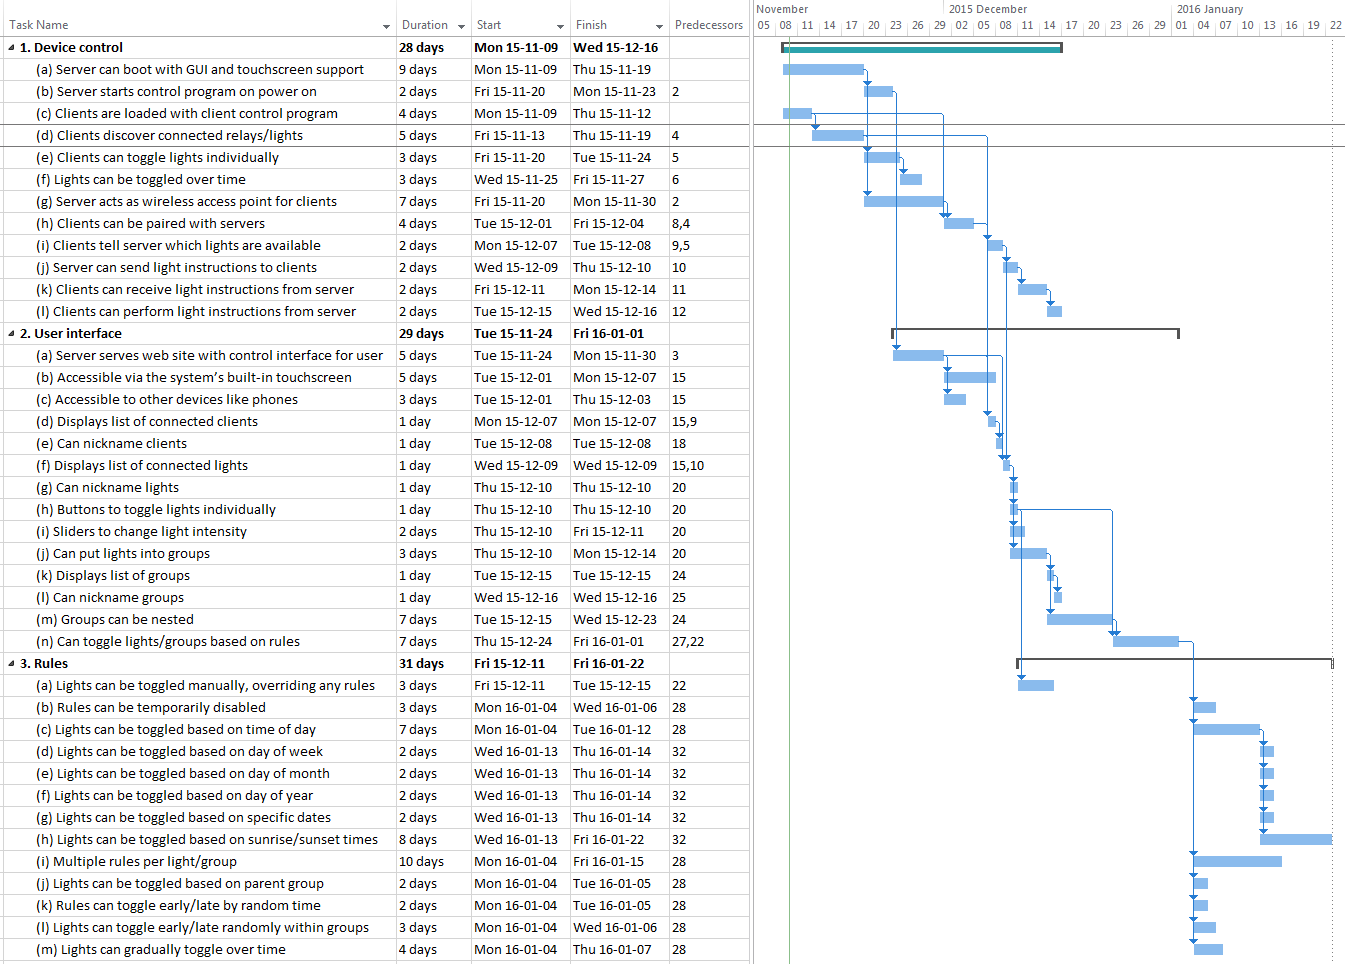
\includegraphics[width=1.0\textwidth]{ganttchart-original.png}
\end{sidewaysfigure}

\pagebreak

\section{Updated Requirements}
Since the original requirements document, only three of our requirements have
been updated, and all for the same reason; they were made into stretch goals
due to hardware limitations.

\begin{tabular}{ l p{7cm} p{2cm} p{6cm} }
    & \textbf{Requirement} & \textbf{Result} & \textbf{Comments} \\
    1f & Lights can be toggled over a user-specified period of time, e.g. a light can gradually turn on and grow brighter over the course of 30 seconds. & Changed to stretch goal. & We decided that this functionality was not possible with the provided relays, which can only toggle lights on or off, not vary their intensity.\\
    2i & The web interface contains sliders for each light that can be used to change the intensity of lights individually. & Changed to stretch goal. & We decided that this functionality was not possible with the provided relays, which can only toggle lights on or off, not vary their intensity.\\
    3m & Lights/groups can be set to gradually dim/brighten over a set period of time.  For example, lights can turn on and gradually brighten from sunset to 30 minutes after sunset, after which they are at full brightness. & Changed to stretch goal. & We decided that this functionality was not possible with the provided relays, which can only toggle lights on or off, not vary their intensity.\\
\end{tabular}

\subsection{Updated Gantt Chart}

Gantt chart available at our project SharePoint website:
%\url{https://oregonstateuniversity-my.sharepoint.com/personal/rettigs_oregonstate_edu/capstone22_project/_layouts/15/start.aspx#/Lists/Tasks/gantt.aspx}
%\begin{sidewaysfigure}
%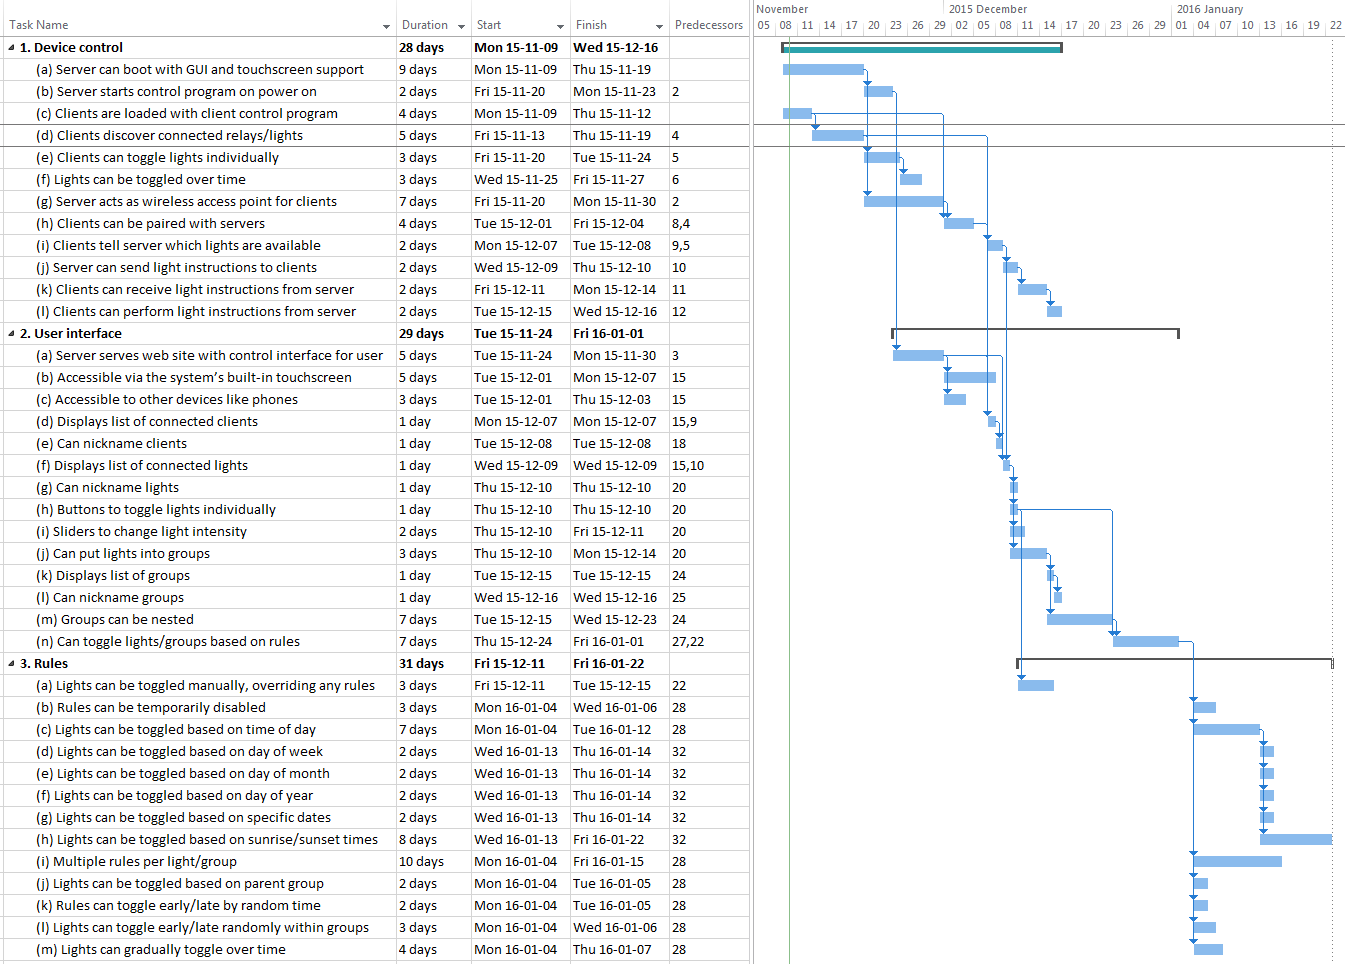
\includegraphics[width=1.0\textwidth]{ganttchart-original.png}
%\end{sidewaysfigure}

\section{Design Document}
\subsection{Introduction}

In the twenty-first century, your home should be smart and responsive. An
automated home should be able to control appliances such as lights through
single-board computer units that have Internet connectivity. Many commercial
options exist, such as those from Nest Labs, but such devices are prohibitively
expensive for most consumers, especially for simple tasks such as lighting
automation. This project aims to provide a low-cost alternative for simple home
automation, for devices like lights and garage door openers. Using a low-cost
embedded computer such as the Raspberry Pi and cheap wireless communication
modules such as the ESP8266, this project will provide a cheap, easy-to-install
home automation system.

The project is called ``Not Exactly the Internet-of-Things'' because it's not
designed as a typical IoT product. The network is entirely local, not worrying
about an external connection to the Wide Area Network. Some additional
components such as consulting an external API could be considered, but that's
an addon to the finished product. As it is made as a home application, it is
readily accessible through smartphones and web interfaces. With a clean user
interface that enables both manual control and automation profiles, the
application will require a minimal learning curve and be simple to set up.  

\subsection{Design View}

The aim of this project is to create a home lighting automation system that is
inexpensive, wireless, and easy to use. The user of this product should the
following features:

\begin{enumerate}
    \item Lights and Groups
    \begin{enumerate}
        \item The lights can be controlled from the built-in touchscreen on the
            control unit, or a mobile device such as a phone, tablet, or laptop
        \item Lights can be put into ``groups'' so that they can be controlled
            all at once
        \item Groups can also be nested into other groups to create hierarchies
            of lights, in order to control many lights at once
        \item The user will be able to nickname lights and light groups
        \item The intensity of each light can be adjusted using a slider
    \end{enumerate}
    \item Rules / Types of Control
    \begin{enumerate}
        \item Lights can be toggled on and off manually, but they can also be
            set to be activated on specific schedules using ``rules''
        \item Rules can be set for lights or groups of lights
        \item There are 6 main types of schedules that rules can trigger on
        \begin{enumerate}
            \item Time of day (e.g. ``turn on at 8pm and turn off at 6am'')
            \item Day of week (e.g. ``turn on during Wednesdays'')
            \item Day of month (e.g. ``turn on every 1st of the month'')
            \item Day of year (e.g. ``turn on every January 1st'')
            \item Specific dates (e.g. ``turn on from Dec. 24th at 2am to Dec
                27th at 8pm'')
            \item Sunrise / sunset (e.g. ``turn on when the sun sets, turn off
                when the sun rises'')
        \end{enumerate}
        \item Multiple rules can be applied to each light or group of lights by
            using AND or OR logic
        \item Lights can be toggled based on the toggle state of its parent
            group
        \item Rules can be enabled or disabled temporarily
        \item Lights or groups can be set to gradually dim/brighten over a set
            period of time instead of toggling
    \end{enumerate}
    \item Stretch Goals
    \begin{enumerate}
        \item The system can control devices other than just lights:
        \begin{enumerate}
            \item Garage door openers
            \item Music players
            \item Holiday decorations
            \item Sprinkler systems
        \end{enumerate}
        \item The web interface is accessible over the Internet (Instead of
            only on the local network)
        \begin{enumerate}
            \item The interface is accessible for only the homeowner or
                authorized individuals
            \item The interface hosted on a remote server if the user does not
                want to deal with port forwarding their home network.
        \end{enumerate}
        \item Additional types of triggers for rules
        \begin{enumerate}
            \item Weather conditions (e.g. lights can turn on automatically if
                it starts raining)
            \item Schedule in a Google calendar
            \item Moon position or other celestial data (e.g. lights could turn
                off during a full moon or solar eclipse for better viewing)
            \item Motion sensors (e.g. lights turn on when someone walks up to
                the front door)
            \item Light sensors (e.g. lights turn off at a certain brightness
                level)
            \item Moisture sensors (e.g. lights turn on when it's wet outside)
            \item Sound sensors (e.g. lights turn on after a loud noise, or
                strobe to the beat of music that is playing)
        \end{enumerate}
    \end{enumerate}
\end{enumerate}

\subsection{Design Viewpoints}

We will be using a wide variety of open source technologies and inexpensive
hardware to provide a low-cost home automation system. We will be using a
varied set of tools to accomplish our goal, including:

\begin{enumerate}
    \item The Yocto Project 
    \begin{enumerate}
        \item The Yocto Project is a kernel building system designed for
            embedded systems. It easily incorporates additional features and
            custom packages directly from Git repositories. It makes it easy to
            build a customized image with only exactly what we want and no
            unnecessary packages \cite{yocto}. It also allows us to customize
            elements of the kernel such as startup scripts in init.d, kernel
            modules, and network scripts \cite{flask}. The kernel will be
            compiled for the Raspberry Pi and copied to an SD card using
            Yocto's filesystem script.
    \end{enumerate} 
        \item Raspberry Pi 2
    \begin{enumerate}
        \item The Raspberry Pi 2 is an ARMv7-processor-based microcomputer
            designed for educational and embedded projects \cite{raspi}. We
            will use it as a low-cost server solution for the lighting
            automation system. It can serve as the web server running NGINX and
            transmit TCP commands to the ESP8266 Wi-Fi modules \cite{nginx}.
            The Pi will be outfitted with a 320x280 TFTLCD display
            \cite{tftlcd} so that the interface for control can be accessed
            directly.  The Pi will also act as a wireless router for the plug
            units to connect to, and run a DHCP server to distribute IP
            addresses to the plug units.
    \end{enumerate} 
        \item ESP8266
    \begin{enumerate}
        \item The ESP8266 is a self-contained SoC (System on a Chip) that has a
            built-in Wi-Fi radio \cite{esp8266}. Our module is outfitted with
            custom firmware, written in Lua and flashed to the device using the
            Arduino IDE, that allows the module to automatically connect to the
            Raspberry Pi (control unit) that acts as a WAP (Wireless Access
            Point) \cite{lua}. The board we have is designed to connect to an
            electronic relay using jumper cables. Using simple TCP commands,
            the board will flip the relay pins on and off \cite{relay}.
    \end{enumerate}
\end{enumerate}

\subsection{User Experience}

The final deliverable of a commercial version of this product would likely
include the following:

\begin{itemize}
    \item A central control unit consisting of the Raspberry Pi, its power
        cable, the touchscreen module, a case, and an SD card with the server
        software preloaded onto it.
    \item One or more plug units which would likely resemble a power strip,
        with each plug being individually controllable by the system.
\end{itemize}

To set up the system, the user simply plugs both the control unit and the plug
unit(s) into wall power.  The plug units will preconfigured to connect to the
control unit.  The user can then plug devices into the plug units, such as
lamps, and the display on the control unit will update itself automatically
with a list of lights.  The lights can have either numbered (e.g. ``Zone 1,
Light 1'') or randomized but memorable names by default (e.g. ``Blue Koala'')
which can be later edited through the web interface.  To access the web
interface, the user connects to the Wi-Fi network provided by the control unit
using the credentials included with the manual, or perhaps printed on the
control unit itself.  They then open a web browser and connect to a specific
URL, provided to the user with the Wi-Fi password.  From the web interface, all
features are accessible, such as renaming lights, creating light groups, and
applying rules for when to toggle lights.

\subsection{Testing}

To test the functionality and correctness of our system, we will test the
various components both individually and when integrated with other components:

\begin{itemize}
    \item We plan to test the wireless communication capabilities of the system
        by attempting to send packets between the control unit and plug units
        at varying distances and in varying environments, including open and
        walled areas.  Ideally, the range should be great enough to fully cover
        the average American house/apartment.  Once this is complete, it will
        likely not need to be changed or extended much, reducing the need for
        regression testing.
    \item We plan to test the actual light toggling (as performed by the plug
        units) manually.  Once this is complete, it will likely not need to be
        changed or extended much, reducing the need for regression testing.
    \item We plan to test the functionality of the touchscreen interface
        through manual human interaction testing.  Once this is complete, it
        will likely not need to be changed or extended much, reducing the need
        for regression testing.
    \item We plan to test the functionality of the web interface through a
        combination of manual human interaction testing, automated API-driven
        testing, and automated GUI testing (using a platform such as Selenium).
        The plug units can send back acknowledgement packets to confirm what
        actions they took in response to the tests, allowing nearly complete
        integration tests to be performed automatically when changes are made
        to the control program and web interface.  These automated tests will
        help prevent regressions as new features are developed and save time in
        ensuring the correctness of the system.
\end{itemize}

\subsection{Timeline}
{\renewcommand{\arraystretch}{0.8}
\begin{tabular}{ | l | l | }
   \hline
   \textbf{Device control} & \textbf{Due Date} \\ \hline

   Server can boot with GUI and touchscreen support & Thu 11/19/15 \\ \hline
   Server starts control program on power on & Mon 11/23/15 \\ \hline
   Clients are loaded with client control program & Thu 11/12/15 \\ \hline
   Clients discover connected relays/lights & Thu 11/19/15 \\ \hline
   Clients can toggle lights individually & Tue 11/24/15 \\ \hline
   Lights can be toggled over time & Fri 11/27/15 \\ \hline
   Server acts as wireless access point for clients & Mon 11/30/15 \\ \hline
   Clients can be paired with servers & Fri 12/4/15 \\ \hline
   Clients tell server which lights are available & Tue 12/8/15 \\ \hline
   Server can send light instructions to clients & Thu 12/10/15 \\ \hline
   Clients can receive light instructions from server & Mon 12/14/15 \\ \hline
   Clients can perform light instructions from server & Wed 12/16/15 \\ \hline
   
   \textbf{User Interface} & \\ \hline
   
   Server serves web site with control interface for user & Mon 11/30/15 \\ \hline
   Accessible via the system’s built-in touchscreen & Mon 12/7/15 \\ \hline
   Accessible to other devices like phones & Thu 12/3/15 \\ \hline
   Displays list of connected clients & Mon 12/7/15 \\ \hline
   Can nickname clients & Tue 12/8/15 \\ \hline
   Displays list of connected lights & Wed 12/9/15 \\ \hline
   Can nickname lights & Thu 12/10/15 \\ \hline
   Buttons to toggle lights individually & Thu 12/10/15 \\ \hline
   Sliders to change light intensity & Fri 12/11/15 \\ \hline
   Can put lights into groups & Mon 12/14/15 \\ \hline
   Displays list of groups & Tue 12/15/15 \\ \hline
   Can nickname groups & Wed 12/16/15 \\ \hline
   Groups can be nested & Wed 12/23/15 \\ \hline
   Can toggle lights/groups based on rules & Fri 1/1/16 \\ \hline
   
   \textbf{Rules} & \\ \hline
   
   Lights can be toggled manually, overriding any rules & Tue 12/15/15 \\ \hline
   Rules can be temporarily disabled & Wed 1/6/16 \\ \hline
   Lights can be toggled based on time of day & Tue 1/12/16 \\ \hline
   Lights can be toggled based on day of week & Thu 1/14/16 \\ \hline
   Lights can be toggled based on day of month & Thu 1/14/16 \\ \hline
   Lights can be toggled based on day of year & Thu 1/14/16 \\ \hline
   Lights can be toggled based on specific dates & Thu 1/14/16 \\ \hline
   Lights can be toggled based on sunrise/sunset times & Fri 1/22/16 \\ \hline
   Multiple rules per light/group & Fri 1/15/16 \\ \hline
   Lights can be toggled based on parent group & Tue 1/5/16 \\ \hline
   Rules can toggle early/late by random time & Tue 1/5/16 \\ \hline
   Lights can toggle early/late randomly within groups & Wed 1/6/16 \\ \hline
   Lights can gradually toggle over time & Thu 1/7/16 \\ \hline
\end{tabular}
}
\subsection{Changes to the Design Document}

Over the course of the year, there were a few changes to the project that had
to be made to allow for new problems that came up when implementing some of the
features specified in the document. The only change that we have made to the
design document since it was created was that we had to remove the lines that
stated ``The intensity of each light can be adjusted using a slider'', and
``Lights or groups can be set to gradually dim/brighten over a set period of
time instead of toggling.'' This had to be done because relays only allow us to
have two states, and unless we used a different implementation and way to
connect to the lights, there is physically no way for us to do dimming or
brightening.

\section{Technology Review}
\subsection{Client}

Victor Hsu\\
Oregon State University\\
Phone: 541-737-4398\\
Email: hsuv@onid.orst.edu

\subsection{Problem Statement}

Outdoor lighting seems like a simple problem to solve, but the solutions on the
market today are less than ideal.  The standard transformer/timer combos
available in the big box stores are rudimentary and clunky at best (constantly
needing to be adjusted for the changing sunset and sunrise times), but are
reasonably priced. The new-generation smart apps for home automation are
flexible and fancier, but are quite spendy and lock you into a specific
protocol.  So why not use an open platform running on commodity hardware?  Easy
to use, reasonably priced, and highly customizable--that is our goal. \\

\subsection{Project Description}

Our system will consist of a wireless network of tiny “client” computers that
each control up to 4 sets of lights and are controlled by a central "server"
computer, which will automatically send out commands to the clients when it's
time to turn on or off.  The central node will run a control program that can
be easily accessed via a touch screen, a web browser, or a mobile device, where
the user can locally or remotely control each light individually.  Want your
lights to turn on at sunset and then dim gradually as the sun rises?  Simple.
Want your lights to flash when you're throwing a party?  Just press a button.
The control interface will allow users to easily set "rules" for what their
lights do and when, depending on the time of day, the sun/moon position, and
potentially even triggers such as weather conditions or calendar dates.  This
system will be easily extensible to potentially control other devices as well,
such as garage doors, sound systems, and more. \\
\hypersetup{linkcolor=blue}
\subsection{Pieces}

\begin{enumerate}
    \item OS for the PI
        \begin{enumerate}
            \item Raspbian \\
                Custom built for the PI, this operating system would provide many important features, and be a solid foundation to run on. Installation is very straightforward, and it has support all across the Internet. This means that the Pi would have to run the entire Raspbian operating system, so there will be many utilities we don't need that will be included anyway. The image is easily acquired and it can be burned to a SD card and booted straight away. It will likely require heavy configuration to get all the necessary services running and the extra ones to never run.
            \item Yocto meta-recipe \\
                We will not need all of the fancy features that Raspbian offers, and one way we can strip our OS down to the features we need is by building a Linux system using Yocto. The Yocto build system is complicated, but our group has experience building layers for various images. It will allow us to build a custom distribution with every package we need, init.d scripts, and service scripts for only the services we need. It will require build time, and time to burn to installation media. Kevin noted that we could get a build server for the project by the end of the term, which would give us good hardware for Yocto builds. 
            \item OpenWRT \\
                An open source router firmware package that allows embedded devices to perform complicated network tasks. Only recently was it recompiled to work with the Raspberry Pi. Our collective experience with the firmware is limited, so it would have an exceptional learning curve. It looks like it would be able to handle all the services we would need, but there isn't a whole lot of flexibility for other additions. It's also very difficult to debug or run tests with. 
        \end{enumerate}
        We have decided to use a Yocto build of Linux for the final build. This decision was made since the Yocto build will only contain exactly what we need, will allow us to easily incorporate new packages with the recipe system, and can be easily shared on our Github repository as a meta-layer for others to build. Proof of concept builds will just use Raspbian with the packages installed.
    \item Server Program Implementation
        \begin{enumerate}
            \item Python / MicroPython \\
            The ESP8266 can run MicroPython for GPIO access, making Python the obvious choice for the server program as well. Using Python's socket API, we can easily connect the devices and execute code to work with the GPIOs. The overhead of Python is minimal when considering the ease of use, and MicroPython was practically designed for the ESP8266, so there's lots of support available. Installing it is as simple as flashing a binary to the ESP8266, and the Python shell is supported. However, we would likely load in a Python script to handle incoming commands from the server. The ESP8266 has sufficient storage for one large Python script.
            \item C / libmraa \\
            Running the system through C is possible, thanks to \href{https://github.com/intel-iot-devkit/mraa}{libmraa} which provides useful abstractions from the /sys/class/gpio and puts it into easy-to-use C libraries. While we could use these libraries, the Python variant provides an easier interface with only slightly more overhead. Additionally, the library contains SWIG-generated wrappers for a variety of languages, including Python, C++, and Perl. The repository is maintained by Intel's IoT Development team, and our team has contribution experience with libmraa. 
            \item sysfs \\
            The most direct, but perhaps least reliable method is to just use the sysfs interface. This involves doing things like echoing values into files and reading the raw files for values. For instance, accessing the SPI interface for a device registered with major number 0 would look like: \verb|cat /sys/class/spi_master/spi0/spi0.0/iio:device0| which is not ideal or clean. Additionally, it could break if we try to use it on systems with different sysfs layouts. It would be useful to use sysfs for testing, but we should not use bash scripts like this for our final product. 
        \end{enumerate}
        We have decided to use Python and MicroPython because of compatibility issues and ease-of-use for the devices. Python will run on both the ESP8266 and the Raspberry Pi with all the libraries we need to run the software. Our concerns about overhead are minuscule since the Python will be executing very simple code; it is just interacting with a relay switch. It will mesh well with our web interface, so we'll be using it as a CGI script in the web server.
    \item Web Site Implementation
        \begin{enumerate}
            \item JavaScript \\
            An easy language to work with, Javascript will allow us to use many different, responsive templates such as react.js and node.js for control. Node even has wrappers for sysfs functionality which may even allow us to deploy it on the ESP8266 devices for remote control. Using JS for the web interface would offload the majority of work from the Pi to the web browser, which could be useful depending on the complexity of our interface. If we end up using a GPIO abstraction library such as libmraa, it should be noted that most of them have wrappers to Javascript code.
            \item Django \\
            A web framework known best for rapid deployment, we could examine this technology as a way to power our entire web interface and backend system. It would have a longer ramp-up time since none of our group members are fully comfortable with Django. However, if we decide that the ramp-up time is worth it, we could see this platform as an all encompassing management tool. Django is well-supported, but does have large learning curve and would require exhaustive group research to understand the entire system. 
            \item PHP \\
            The hypertext preprocessor is, at first glance, perhaps not the best system to run our backend off of, but we're considering it for a few reasons. It can execute our CGI scripts with the mod\_php module for the web server, our group has significant working experience with the language, and it just works out of the box. It may require additional configuration, but from a 10,000 foot view it accomplishes all the tasks we need. It can mesh well with a wide variety of other technologies we may end up using, and is highly modular.
        \end{enumerate}
        We have decided to use the HTML/JS/PHP stack for our project, which means we'll be building a system from the ground up. We can point the Javascript to the CGI files to execute the Python that will change the relays at the remote end, use PHP for the web backend and database access, and use HTML for the pages themselves (although this one will likely just be generated through the PHP code too) to create our full web server stack. This does not rule out us using other technologies such as node or Django as a subsystem.
    \item Server/Client Communication
        \begin{enumerate}
            \item AD-HOC \\
            In this communication method, the devices are configured for AD-HOC mode, or a packet-radio system. The wireless adapters need to be able to support AD-HOC mode and be set to a specific channel and IP range. Given the difficulty we've had with AD-HOC networks in the past, we'll maybe try to avoid this mode, but it would be useful as a proof-of-concept for socket communication. However, this is likely not a long-term solution.
            \item Central WAP \\
            We would configure one Raspberry Pi as a central Wireless Access Point and have the ESP8266 units connect to it as wireless clients. The advantage to this mode is that we could use the Raspberry Pi to connect to the Internet to perform tasks such as talking to the Wunderground API, which is not possible in AD-HOC mode. This would require that the Pi run a DHCP server, along with other routing services.
            \item CAS \\
            A Central Authority Service model leans more toward the well-defined Internet of Things model. All of our devices rely on an external server for almost all their actions. It would coordinate between the devices, actually store all the data and perform all the heavy lifting, relying on the Pi and ESP8266 devices only for GPIO access. A drawback to this model is the additional server we'd need to configure and rely on, especially since the system would stop working if the server ever becomes inaccessible.
        \end{enumerate}
        We have decided to use the WAP model because it provides the benefits of the AD-HOC and CAS models without all the additional configuration burdens. A Yocto meta-recipe for the Pi's WAP functionality would be simple, and connections between the ESP8266 devices would become a trivial task. This does mean the Pi has to run extra services (like DHCP), but it should be more than capable of running the limited services we will require of it.
\end{enumerate}

\subsection{Changes to the Technology Review}

The only large change that we made in regard to the decisions in our technology review was that for the website, we used no PHP to modify the database, and instead used a python Object Relational Mapper (ORM) called SQLAlchemy. Additionally, we used a python web framework for our website called Flask. Combined, these allowed for much cleaner code and a much easer to manage database access.

\section{Blog}
\subsection{Fall Update 3}
Progress since last week:
\begin{itemize}
   \item We have finished the requirements document after having our client review it.
   \item We received our Raspberry Pi and touchscreen hardware.
\end{itemize}
Problems:
\begin{itemize}
   \item No problems this week.
\end{itemize}
Plans for the coming week:
\begin{itemize}
   \item Begin working on the Pi starting with an operating system and then branching out to communication between the devices and touchscreen capabilities.
\end{itemize}
Blog Date: 10-29-15


\subsection{Fall Update 4}
Most of what we did this week involved trying to get a functioning proof of concept for our project, which turned out to be filled with more problems than anticipated. We began to investigate software packages and technologies that would help us meet the requirements outlined on our document. We will hopefully have a functional proof-of-concept by the next week.\\
Progress since last week:
\begin{itemize}
   \item Tested the devices with various wireless networking methods, including ad-hoc and in access-point mode
   \item Continued to develop our documents such as the technical requirements and elevator pitch
\end{itemize}
Problems:
\begin{itemize}
   \item The ad-hoc system did not work as expected due to the USB WiFi adapters we were using, and we had to reevaluate​ our network implementation
\end{itemize}
Plans for the coming week:
\begin{itemize}
   \item Continue to develop a proof-of-concept, working with a new structure with the wireless components that will function to expectations.
\end{itemize}
Blog Date: 11-5-15

\subsection{Fall Update 5}
Progress since last week:
\begin{itemize}
   \item We now have a working proof of concept where the Pi is able to wirelessly communicate to the ESPs and cause each of the connections on the relays to be activated individually.
   \item Completed technology review and revision of requirements document.
   \item Started on expo poster.
\end{itemize}
Problems:
\begin{itemize}
   \item No real problems other than having to revise the requirements document to be more detailed and fine-grained.
\end{itemize}
Plans for the coming week:
\begin{itemize}
   \item Finish Poster
   \item Revise elevator pitch
   \item Demonstrate proof of concept
   \item Possibly attach actual lights to the relay rather than just using the relay's LEDs to see which switches are enabled.
\end{itemize}
Blog Date: 11-13-15

\subsection{Fall Update 6}
Progress since last week:
\begin{itemize}
   \item Our proof of concept is now portable, and booting the pi connects it to the ESP8266 module and cycles the lights on the relay.​ It has also been shown to the TA.
   \item Finished expo poster
   \item Re-wrote elevator pitch
\end{itemize}
Problems:
\begin{itemize}
   \item No real problems this week
\end{itemize}
Plans for the coming week:
\begin{itemize}
   \item Continue to develop the proof of concept, possibly by adding actual lights to the relay instead of the LED's.
   \item Present the elevator pitch​
\end{itemize}
Blog Date: 11-19-15

\subsection{Fall Update 7}
Progress since last week:
\begin{itemize}
   \item We have connected actual lights to our relay and verified that they can be toggled on/off.
   \item We have presented our elevator pitch.
   \item We have begun learning how to use Flask for our website.
\end{itemize}
Problems:
\begin{itemize}
   \item No real problems this week
\end{itemize}
Plans for the coming week:
\begin{itemize}
   \item Work on our design document​
   \item Become more familiar with Flask and potentially start on the website
      Use the Yocto build server to build the new system rather than using Raspbian.
   \item Work on progress report
\end{itemize}
Blog Date: 11-28-15


\subsection{Fall Update 8}
Progress since last week:
\begin{itemize}
   \item We retrieved our build server from Kevin and installed Linux. We also installed the Yocto build system and built core-image-minimal to verify that it works.
   \item We booted the Raspberry Pi with core-image-minimal to verify that the images would work
   \item We investigated options for connections and user experiences, and decided on a wireless connection method for our system
   \item We completed our design document and ran it by our TA. We also continued work on the progress report.
\end{itemize}
Problems:
\begin{itemize}
   \item We had a bit of a confused discussion on the user experience complexity and the wireless communication methods we would use, as we did not know the expectations for ease-of-use. We contacted Victor and had our questions answered.
\end{itemize}
Plans for the coming week:
\begin{itemize}
   \item Work on our report
   \item Over break, start to build the web framework with Flask.
\end{itemize}
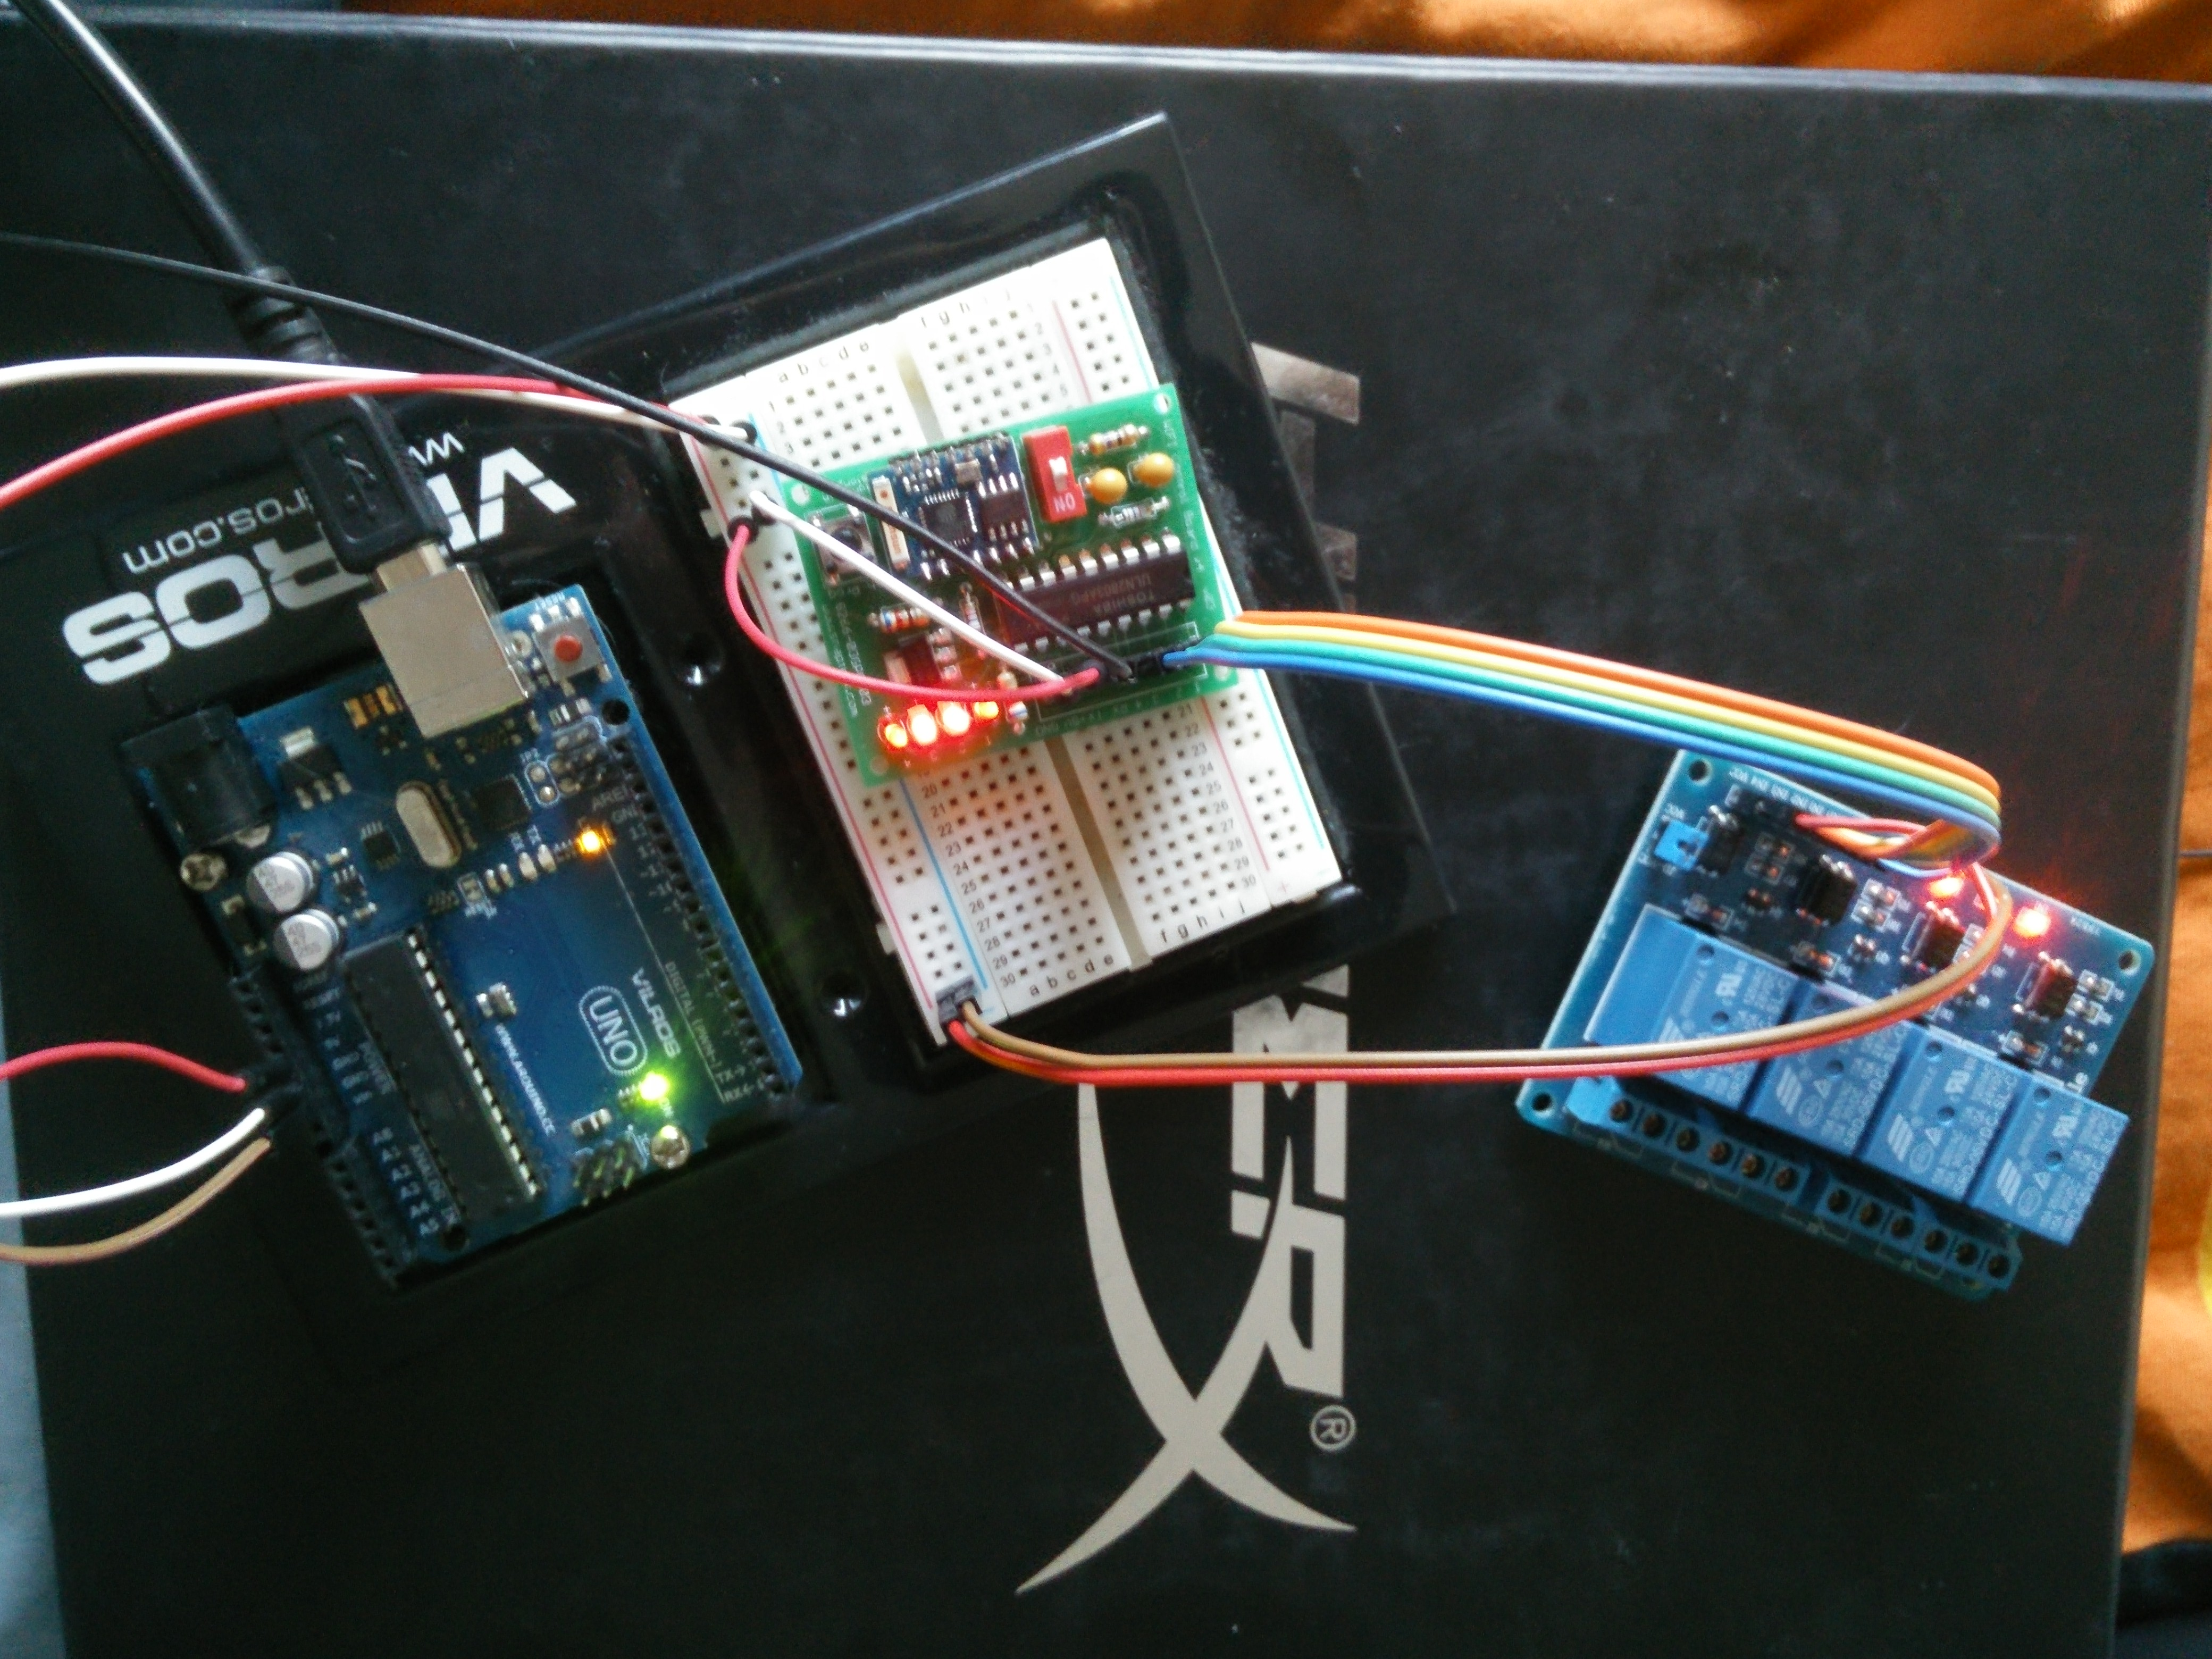
\includegraphics[scale=0.05]{circuit1}\\
Blog Date: 12-4-15

\subsection{Winter Update 1}
Over the break, our group refreshed our working knowledge of Flask, configured our new device for our Yocto build server and continued testing with the Raspberry Pi. We resumed work on the project and plan to meet during the weeks throughout the term to coordinate work, although most of our work will happen outside of our meetings. \\
Progress over break:
\begin{itemize}
   \item Reviewed Python Flask to be better prepared to start working on it to build our web interface.
   \item Configured the Raspbery Pi with software to run the web interface such as the ISC DHCP server and a basic DNS server.
   \item Used Hostapd and wpa\_supplicant to have the Wifi adapter on the Pi broadcast an access point.
\end{itemize}
Week 1 work:
\begin{itemize}
   \item Met to discuss web layout, decided on various Javascript libraries to run the application
   \item Continued to develop software configuration for the Raspberry Pi and the corresponding Yocto image.
\end{itemize}
Problems:
\begin{itemize}
   \item Some minor nonviolent disagreements on design for the front end of the application​
\end{itemize}
Plans for the coming week:
\begin{itemize}
   \item Continue development of front end application
   \item Finish back-end scripts to send the commands to the ESP8266 module
   \item Finish Python ISC-DHCP autodiscovery scripts
\end{itemize}
Blog Date: 1-8-16

\subsection{Winter Update 2}
Progress since last week:
\begin{itemize}
   \item Changed requirements document to show that adjusting the brightness of lights is now a stretch goal. (requirements 1f, 2i, and 3m)
   \item Created our first way to send the TCP command for turning on and off the lights.
   \item Added database capability for the ESP devices.
   \item Reformatted the layout of the website to be more compartmentalized and manageable.
   \item Added python data structures for groups and lights
\end{itemize}
Problems:
\begin{itemize}
   \item We realized that we would not be able to accomplish our goal of being able to adjust the brightness of the lights with the hardware we have available. We changed this goal to a stretch goal in the requirements document.
\end{itemize}
Plans for the coming week:
\begin{itemize}
   \item Continue development of front end application
   \item Work more on connecting the website to the functions of the hardware
\end{itemize}
Blog Date: 1-15-16

\subsection{Winter Update 3}
Progress since last week:
\begin{itemize}
   \item Added interface to add and view current connected ESP8266 devices, along with error handling.
   \item Performed minor formatting and usability updates to the front page.
   \item Created a basic Advanced page to accept dates/times for when to turn lights on/off and a basic query string that is able to live update via Javascript.
\end{itemize}
Problems:
\begin{itemize}
   \item No notable problems this week.
\end{itemize}
Plans for the coming week:
\begin{itemize}
   \item Malcolm plans to work on making the front page of the site more usable by allowing the editing of names, the creation/deletion of groups, and the sending of reordering operations to the server from the web browser.
   \item Sean plans to continue work on the Advanced page for creating rules for lights, including creating a proper query string and actually sending the updates back to the server.
\end{itemize}
Blog Date: 1-22-16

\subsection{Winter Update 4}
Progress since last week:
\begin{itemize}
   \item Decided on a database layout for creating and displaying light groups on the front page of the site.
   \item Continued to add support for the advanced page and improving the Javascript creating the custom queries.
   \item Added login functionality and created a default user when the database is created. We'll actually apply the security to the pages when the project is near completion.
\end{itemize}
Problems:
\begin{itemize}
   \item Minor disagreements on what to use for the group table structure, but resolved during Thursday's meeting.
\end{itemize}
Plans for the coming week:
\begin{itemize}
   \item Malcom will add the group display functionality to the front page, and will apply the \textit{jquery\_editable} functions to the group entries to allow easy editing of group attributes.
   \item Sean will flesh out the logic generation subsystem as it interacts with the new light group management so that manual overrides are possible without disruption customized schedules.
   \item Evan will finish the devices display and modification page by applying the \textit{jquery\_editable} package to it and will then work on the group layout with Malcom.
\end{itemize}
\subsection{Winter Update 5}
Progress since last week:
\begin{itemize}
   \item Re-Wrote querybuilding on the server and started on the client's querybuilding.
   \item Finalized the database schema and the flask sql-alchemy object relational model format.
   \item Additional changes to the advanced page
\end{itemize}
Problems:
\begin{itemize}
   \item No major problems this week.
\end{itemize}
Plans for the coming week:
\begin{itemize}
   \item We will work on and complete the Midterm Progress Report, as well as the accompanying video.
\end{itemize}
Blog Date: 2-8-16

\subsection{Winter Update 6}
Progress since last week:
\begin{itemize}
   \item Updated the formatting, fixed general bugs, and cleaned up the code for the website in both the advanced page and the main page
   \item Finished the query builder for the advanced page
   \item Rules now appear on the side when created
   \item Finished both the progress report and the video to go along with it.
\end{itemize}
Problems:
\begin{itemize}
   \item No major problems this week.
\end{itemize}
Plans for the coming week:
\begin{itemize}
   \item We will continue to work on achieving beta-level functionality for all parts of the project
\end{itemize}
Blog Date: 2-12-16

\subsection{Winter Update 7}
Progress since last week:
\begin{itemize}
   \item Implemented sorting on the Flask app's front page for groups
   \item Added JS for deleting groups and adding of new groups
   \item Continued logical development for the advanced page and custom user queries
   \item Fixed some minor styling bugs with custom CSS
\end{itemize}
Problems:
\begin{itemize}
   \item No major problems this week.
\end{itemize}
Plans for the coming week:
\begin{itemize}
   \item Continue working on the advanced user queries
   \item Implement group change interaction with the database on the front page
\end{itemize}
Blog Date: 2-19-16

\subsection{Winter Update 8}
Progress since last week:
\begin{itemize}
   \item Reorganized advanced page layout for usability according to feedback from user study.
   \item Removed ability to apply multiple rules to each light/group to improve usability, since users found the concept of multiple rules per light/group confusing.  No functionality is lost, however, since parent group rules can still be applied, and custom queries can be created that achieve the same result as multiple rules.
      \begin{itemize}
         \item Since each light/group only has one rule now, the rules table was removed from the database and a rule column was added to the light and group tables.
      \end{itemize}
   \item Advanced page now sends rule changes to the server via AJAX, updating the database immediately whenever a change is made.  This negates the need for the user to hit a "save changes" button or the like, which users responded poorly to in the user study.
   \item Fixed bug with deleting groups that have nested group children on the main page.
   \item Fixed additional minor styling bugs, such as with the light/group name editing box on the main page appearing on a new row.
\end{itemize}
Problems:
\begin{itemize}
   \item No major problems this week.
\end{itemize}
Plans for the coming week:
\begin{itemize}
   \item Implement job for re-evaluating rules on startup and periodically, including calculating proper sunset/sunrise times, and then sending updates to each light.
   \item Make further style/usability tweaks to site, including front page and advanced page, such as making buttons bigger, adding help text, fixing alignment of elements, etc.
   \item Create settings page
      \begin{itemize}
         \item Currently, only planned setting is for geographical location for calculating accurate sunset/sunrise times.
      \end{itemize}
   \item Intregation testing
      \begin{itemize}
         \item Starting from an empty database, add a new client device and toggle the lights from the main web UI and through rules.
         \item Test the use of the website on the Pi's touchscreen.
      \end{itemize}
\end{itemize}
Blog Date: 2-26-16

\subsection{Winter Update 9}
Progress since last week:
\begin{itemize}
   \item As we near the end of our project, we have started using Github's issue tracker for all bugs and yet-to-be-implemented features:
      \begin{itemize}
         \item https://github.com/capstone22-Pilight/cs-senior-capstone/issues
      \end{itemize}
   \item Essentially finished beta version of project, completing all high priority issues.
   \item The main portion of the project that was finished was the advanced page and rule system; the advanced page has been reformatted to make it easier to use, and the rule system was overhauled to use custom datetime wrapper objects to elegantly handle early/late toggle times and randomized toggle times.
      \begin{itemize}
         \item We also implemented sunset/sunrise time calculation using the Astral Python module and adding a settings page that allows the user to select their geographic location.
         \item Furthermore, the scheduler that actually runs the rules periodically has been implemented, using the Schedule Python module.
      \end{itemize}
   \item We have performed integration testing involving using all of the main features of the project (e.g. toggling lights manually, using rules, using groups, etc.) on the provided hardware and all of the functionality is there, save for a few minor bugs.
   \item We have updated our poster to reflect the current status of the project.
   \item We have created a slideshow presentation for use as an outline for our final video presentation.
\end{itemize}
Problems:
\begin{itemize}
   \item It was fairly minor, but originally, we had issues with the rule system ignoring manual overrides; whenever a user manually toggled a light, the rule system would overwrite it the next time it ran.
      \begin{itemize}
         \item This was solved by making sure that the overridden state of a light was stored in the database and making rules check if a light is overridden before updating it.
      \end{itemize}
\end{itemize}
Plans for the coming week:
\begin{itemize}
   \item Resolve all medium-priority issues.  Fixing low-priority issues will be our goal next term, as they are mostly minor usability and maintainability improvements that are not necessary for a beta release.
   \item Finish poster and slideshow
   \item Finish video and progress report
\end{itemize}
Blog Date: 3-8-16

\subsection{Winter Update 10}
Progress since last week:
\begin{itemize}
   \item Continued work on isses for the project, including adding new ones since week 9 and resolving outstanding ones
      \begin{itemize}
         \item Total issues currently open: 9 (all low-priority)
         \item 19 issues closed: 11 medium, 3 high priority
      \end{itemize}
   \item The full unit test with the screen, mobile device, and relay connected to LEDs was conducted. The tests revealed bugs that were caught and fixed.
      \begin{itemize}
         \item For instance, we found out that we needed to reverse the logic for generating the TCP commands to make the relay function properly.
      \end{itemize}
   \item We created our presentation video for the physical device and began shooting video for our powerpoint presentation
   \item We finalized our poster after review and submitted the final revision
\end{itemize}
Problems:
\begin{itemize}
   \item The lights on the relay were out of sync, we fixed this by logically flipping the TCP command sent to the ESP module
   \item The override function did not match the requirements document, so Sean revised the override logic to match the requirement.
\end{itemize}
Plans for the coming week:
\begin{itemize}
   \item Finish video and progress report
\end{itemize}
Blog Date: 3-11-16

\subsection{Spring Update 1}
At this point, our project is at a completed stage, but we have identified a few bugs and usability issues that we will spend this term working on.\\
Progress at start:
\begin{itemize}
   \item We met to discuss adding new issues to work on this term as enhancements to the final product. Our first priority is to complete two new medium-level issues before the Expo:
      \begin{itemize}
         \item Create a JS poller so that the lights update on all open pages when the rules or a user changes them.
         \item Change the default names for lights so that they're user-friendly.
      \end{itemize}
   \item Evan has been using the system at home to run his own lights as part of a long term test. The test began on 3/31/16 and will be updated as we get closer to expo.
   \item We added the Yocto layer for the build and the site itself to the Github repo, and will be updating the Readme to add the proper Yocto version and machine type.
\end{itemize}
Problems:
\begin{itemize}
   \item We had no major issues, and since the finished product (minus usability changes and bug fixes) has been demonstrated and is in long-term testing, we don't expect many production issues at this point.
\end{itemize}
Plans for the coming week:
\begin{itemize}
   \item Resolve all medium-priority issues.
\end{itemize}
Blog Date: 4-4-16

\subsection{Spring Update 2}
Progress this week:
\begin{itemize}
   \item We met with our client, Victor, to demonstrate the state of our project and receive feedback.  Some of the suggestions from the meeting include:
      \begin{itemize}
         \item Make sure to account for daylight savings time.
         \item Make rules run more often than every 60 seconds, especially for demos.
         \item Make rules run immediately when rules are changed.
         \item Include a way to simulate time running faster, especially for demos.  This could potentially allow a whole daily cycle to be simulated in just seconds, showing off the rule system in a timely fashion.
         \item Improve our physical demo setup; our current setup involves a breadboard, an extra Arduino for power, and a lot of stray wires; our new plan is to have a small model house made from PCB with the LEDs soldered in and hooked up directly to a 120V to 5V converter.  We also plan to have 2 ESP/relay units for the final demo, which Victor has ordered for us.
      \end{itemize}
   \item We also started work on some of our highest-priority issues, particularly the client-side polling to automatically update light statuses without refreshing, and checks to prevent light statuses from changing if a toggle action failed (such as if the power strip was unplugged or there was wireless interference).
\end{itemize}
Problems:
\begin{itemize}
   \item One problem we had was that during the demo with our client, the rules did not seem to trigger when they should have.  However, we later realized that we had been manually toggling the lights immediately beforehand, which overrode the rules; the behavior was actually intended.  We need to remember this in future demos.  The faster time simulation could help with this since even if we override the lights, the override period will end much more quickly.
\end{itemize}
Plans for the coming week:
\begin{itemize}
   \item Finish and submit final version of expo poster
   \item Complete high priority issues
   \item Prepare model for expo
\end{itemize}
Blog Date: 4-13-16

\subsection{Spring Update 3}
Progress this week:
\begin{itemize}
   \item Added a function to the test branch for the int\_bool conversion to make the code involved with clicking the group buttons cleaner.
   \item Removed the duplicate add\_device function, and cleaned up the original by making better default names.
   \item Started building a rough model house to use at expo using junk pcb.
   \item Started work on the poller which checks the status of the lights and updates them for the client if they have changed.
\end{itemize}
Problems:
\begin{itemize}
   \item Our int\_bool conversion branch is still not toggling all of the lights in a group correctly when one of the group control buttons is pressed
\end{itemize}
Plans for the coming week:
\begin{itemize}
   \item Debug and fix the problem with the int\_bool conversion branch
   \item Continue working on and possibly finish the pcb model house
   \item Polish up the poster so that it can be submitted at the end of next week
   \item Complete high priority issues
\end{itemize}
Blog Date: 4-15-16

\subsection{Spring Update 4}
Progress this week:
\begin{itemize}
   \item Polished the poster and submitted it to the TA for review
   \item Constructed the first prototype for the house model for use at expo (pictured below)
   \item Completed changing entry in database for light status from integers to booleans
   \item Completed the poller to update the switch status across windows.
\end{itemize}
Problems:
\begin{itemize}
   \item No major issues encountered this week
\end{itemize}
Plans for the coming week:
\begin{itemize}
   \item Complete all medium-level issues
   \item Complete the next prototype for the house model for expo
\end{itemize}
Blog Date: 4-24-16

\subsection{Spring Update 5}
Progress this week:
\begin{itemize}
   \item Began work on final report
   \item Finalized our expo poster
   \item Submitted our expo poster for printing
   \item Merged the fix for the Integer to Boolean conversion issue
\end{itemize}
Problems:
\begin{itemize}
   \item No major issues encountered this week
\end{itemize}
Plans for the coming week:
\begin{itemize}
   \item Complete the video for submission next friday
   \item Complete the final report for submission next friday
   \item Resolve all medium level issues
\end{itemize}
Blog Date: 5-6-16

\subsection{Spring Update 6}
Progress this week:
\begin{itemize}
   \item Completed final version of the house/castle we will use at expo for demonstration
   \item Completed and submitted the final report
   \item Completed and submitted the video
   \item Resolved the issue to add reset buttons
\end{itemize}
Problems:
\begin{itemize}
   \item No major issues encountered this week
\end{itemize}
Plans for the coming week:
\begin{itemize}
   \item Continue fixing and resolving all medium level issues
   \item Prepare for expo presentation
\end{itemize}
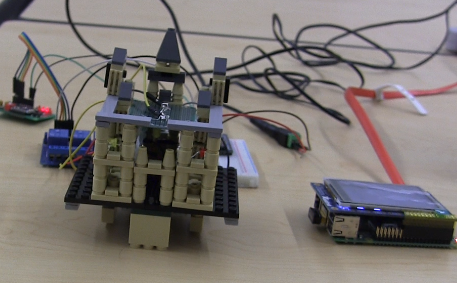
\includegraphics[scale=0.5]{castle}\\
Blog Date: 5-6-16

\subsection{Spring Update 7}
Progress this week:
\begin{itemize}
   \item Bug fixing on Javascript poller
   \item Bug fix on footer section
   \item Completed and submitted the video
   \item Bug fix on reset button
\end{itemize}
Problems:
\begin{itemize}
   \item No major issues encountered this week
\end{itemize}
Plans for the coming week:
\begin{itemize}
   \item Continue fixing and resolving all medium level issues
   \item Create final presentation for Expo
   \item Collect all materials (Evan!) and make sure that no major technical errors will occur at expo
\end{itemize}
Blog Date: 5-14-16

\subsection{Spring Update 8}
Progress this week:
\begin{itemize}
   \item Prepared for Expo by practicing our presentation and fixing any outstanding bugs
   \item Participated in Expo
\end{itemize}
Problems:
\begin{itemize}
   \item No major issues encountered this week
\end{itemize}
Plans for the coming week:
Blog Date: 6-5-16

\subsection{Spring Update 9}
Progress this week:
\begin{itemize}
   \item Recieved 2nd place award for our performance at the Expo
\end{itemize}
Problems:
\begin{itemize}
   \item No major issues encountered this week
\end{itemize}
Plans for the coming week:
Blog Date: 6-5-16

\subsection{Spring Update 10}
Progress this week:
\begin{itemize}
   \item Assigned parts to complete for the final report
\end{itemize}
Problems:
\begin{itemize}
   \item No major issues encountered this week
\end{itemize}
Plans for the coming week:
\begin{itemize}
   \item Complete and submit the final report and presentation
\end{itemize}
Plans for the coming week:
Blog Date: 6-5-16

\section{Poster}
\section{The Project}
\subsection{Design}
\subsubsection{Theory of Operation}
\subsection{Installation}
As part of our installation, we have two modes of putting the image on your Raspberry Pi. These are tailored to users who just want an express installation with no difficulties, and for users who wish to build their own Pilight image from scratch using the Yocto Builder.
\subsection{Express install}
The wiki on Github has a link to a prebuilt image of the Pilight system we had in place at expo. This image is updated using Yocto's autobuilder program Toaster. Once downloaded, it can be installed like any other image for a Raspberry Pi.
\subsubsection{Windows}
Windows will use the graphical utility Win32DiskImager to install our image to the SD card.
\begin{itemize}
   \item Download the image from the Pilight Wiki at \url{https://github.com/rettigs/cs-senior-capstone/wiki}
   \item Insert the SD card into your SD card reader and check which drive letter was assigned. You can easily see the drive letter, such as G:, by looking in the left column of Windows Explorer. You can use the SD card slot if you have one, or a cheap SD adapter in a USB port.
   \item Download the Win32DiskImager program from \url{http://sourceforge.net/projects/win32diskimager/}, which will provide a way to put the image on the SD card
   \item Extract the executable from the zip file and run the Win32DiskImager utility; you may need to run this as administrator. Right-click on the file, and select Run as administrator.
   \item Select the image file you extracted earlier.
   \item Select the drive letter of the SD card in the device box. Be careful to select the correct drive; if you get the wrong one you can destroy the data on your computer's hard disk! If you are using an SD card slot in your computer and can't see the drive in the Win32DiskImager window, try using an external SD adapter.
   \item Click Write and wait for the write to complete.
   \item Exit the imager and eject the SD card.
\end{itemize}
\subsubsection{OSX}
On Macs we can use the command-line utilities for creating our image.
\begin{itemize}
   \item Insert your SD card to an SD card reader
   \item Use the disk reader program to identify your SD card:
      \begin{lstlisting}
      diskutil list
      \end{lstlisting}
   \item Identify the disk (not partition) of your SD card e.g \textit{disk4}, not \textit{disk4s1}
   \item Unmount the SD card
      \begin{lstlisting}
      diskutil unmountDisk /dev/disk<disk# from diskutil>
      \end{lstlisting}
      where \textit{disk} is your BSD name e.g. \textit{diskutil unmountDisk /dev/disk4}
   \item Copy the data to the SD card:
      \begin{lstlisting}
      sudo dd bs=1m if=pilight.img of=/dev/rdisk<disk# from diskutil>
      \end{lstlisting}
      where \textit{disk} is your BSD name e.g. \textit{/dev/disk4}
      \begin{itemize}
         \item This may result in a \textit{dd: invalid number '1m'} error if you have GNU coreutils installed. In that case, just change the \textbf{bs=1m} to \textbf{bs=1M}
      \end{itemize}
\end{itemize}
\subsubsection{Linux}
Our Linux install is similar to OSX, but using Linux tools instead
\begin{itemize}
   \item Run \textit{df} to find where your SD card is mounted:
      \begin{lstlisting}
      df -h
      \end{lstlisting}
      It will be listed as something like \textit{/dev/mmcblk0p1} or \textit{/dev/sdd1}. For later steps, you'll need the name without the partition number, which would change the values to \textit{/dev/mmcblk0} and \textit{dev/sdd}
   \item Unmount the drive. For \textit{/dev/sdd} it would be:
      \begin{lstlisting}
      umount /dev/sdd1
      \end{lstlisting}
   \item Write the data to the SD card. Again for \textit{/dev/sdd} it would be:
      \begin{lstlisting}
      dd bs=4M if=pilight.img of=/dev/sdd
      \end{lstlisting}
   \item Run sync to flush the write cache
      \begin{lstlisting}
      \end{lstlisting}
\end{itemize}

\subsection{Hardware Requirements}
\section{New Technology}
There were several technologies we used that many people in our group were not familiar with, but learning them was not too great of a challenge.

\begin{itemize}
	\item Python \\
	While we had all had experience with python before starting on this project, for most of us this was our first large scale project that was almost entirely Python-based. For most questions we had about syntax particulars, we used the standard \href{www.docs.python.org}{Python Documentation}.
	\item SqlAlchemy \\
	For database managment, we used a Object Relational Mapping (ORM) python library called SqlAlchemy. For information on how to implement it and use it accordingly, we used the \href{www.docs.sqlalchemy.org}{SqlAlchemy Docs} on the SqlAlchemy Website.
	\item Flask \\
	We decided to use Flask as a framework for our website, which ended up being extremely useful, as it allows for a very seamless integration between the front and back ends of our server. As none of us had used Flask before, the \href{www.flask.pocoo.org\/docs}{Flask Documentation} was extremely helpful. Another resource that was useful for learning Flask in a more in-depth sense was \href{blog.miguelgrinberg.com\/post\/the-flask-mega-tutorial-part-i-hello-world}{The Flask Mega-Tutorial}.
	\item Bootstrap \\
	While some people in the group had used bootstrap before, others were new, and even those who were already familiar with it sometimes needed to look up specifics about how to use it. A resource we found useful was the main \href{www.getbootstrap.com}{Bootstrap Documentation}, as well as the \href{www.bootstrap-switch.org}{Bootstrap Switch} page for information on how to use the Switches plugin.
	\item Jquery \\
	The Jquery API proved very useful when writing the javascript for our website. As some of us were new to it and others had used it a decent amount, the \href{www.api.jquery.com}{Jquery Documentation} proved quite useful, especially when using the query functionality.
	\item Yocto \\
	Only one of our group members had used the Yocto build environment before, but he was able to provide the advice that we needed to make our project work.
	\item Firmware \\
	We needed to write firmware to make the ESP 8266 module do what we want. This would have been very obscure and hard to do without a reference of some sort, and the one we found useful was a \href{www.github.com\/nodemcu\/nodemcu-firmware}{github repository} that was fairly well organized. We based our firmware off of this code with some slight modifications.
	\item Google \\
	As always when learning new technology, google proved to be an invaluable resource, as the ability to search the web was very useful indeed.
\end{itemize}
\section{Team Discussion}
\subsection{Evan Steele}
\subsection{Malcolm Diller}
\subsection{Sean Rettig}
\section{Code}
\section{Photos}
\Urlmuskip=0mu plus 1mu\relax
\bibliographystyle{IEEEtran}
\bibliography{end\_report}
\end{document}
